
\chapter{Validierung}

\section{Analyse der spannkraftinduzierten Deformation}\

[explizit Unterschiede FDM und additiv herausstellen mit genauen Angaben über die Deformationen]

Mithilfe dieser Funktion können unterschiedliche Bauteilgeometrien und 
Herstellungsprozesse auf ihre Deformation verglichen werden.

Bei einem additiv gefertigten Metallteil, tritt bei den gleichen Spannungsstufen
eine deutlich kleinere, aber dennoch eine erkennbare Deformation auf.
Zusätzlich ist zu sehen, dass bei verschiedenen Herstellungsprozess, trotz
gleicher Geometrie unterschiedliche Verformungen auftreten.

[vllt expliziter, wo genau tritt die Deformation auf, 
von wie viel Deformation reden wir, was bedeutet das für das Realbauteil]

\begin{figure}[H]
    \centering
    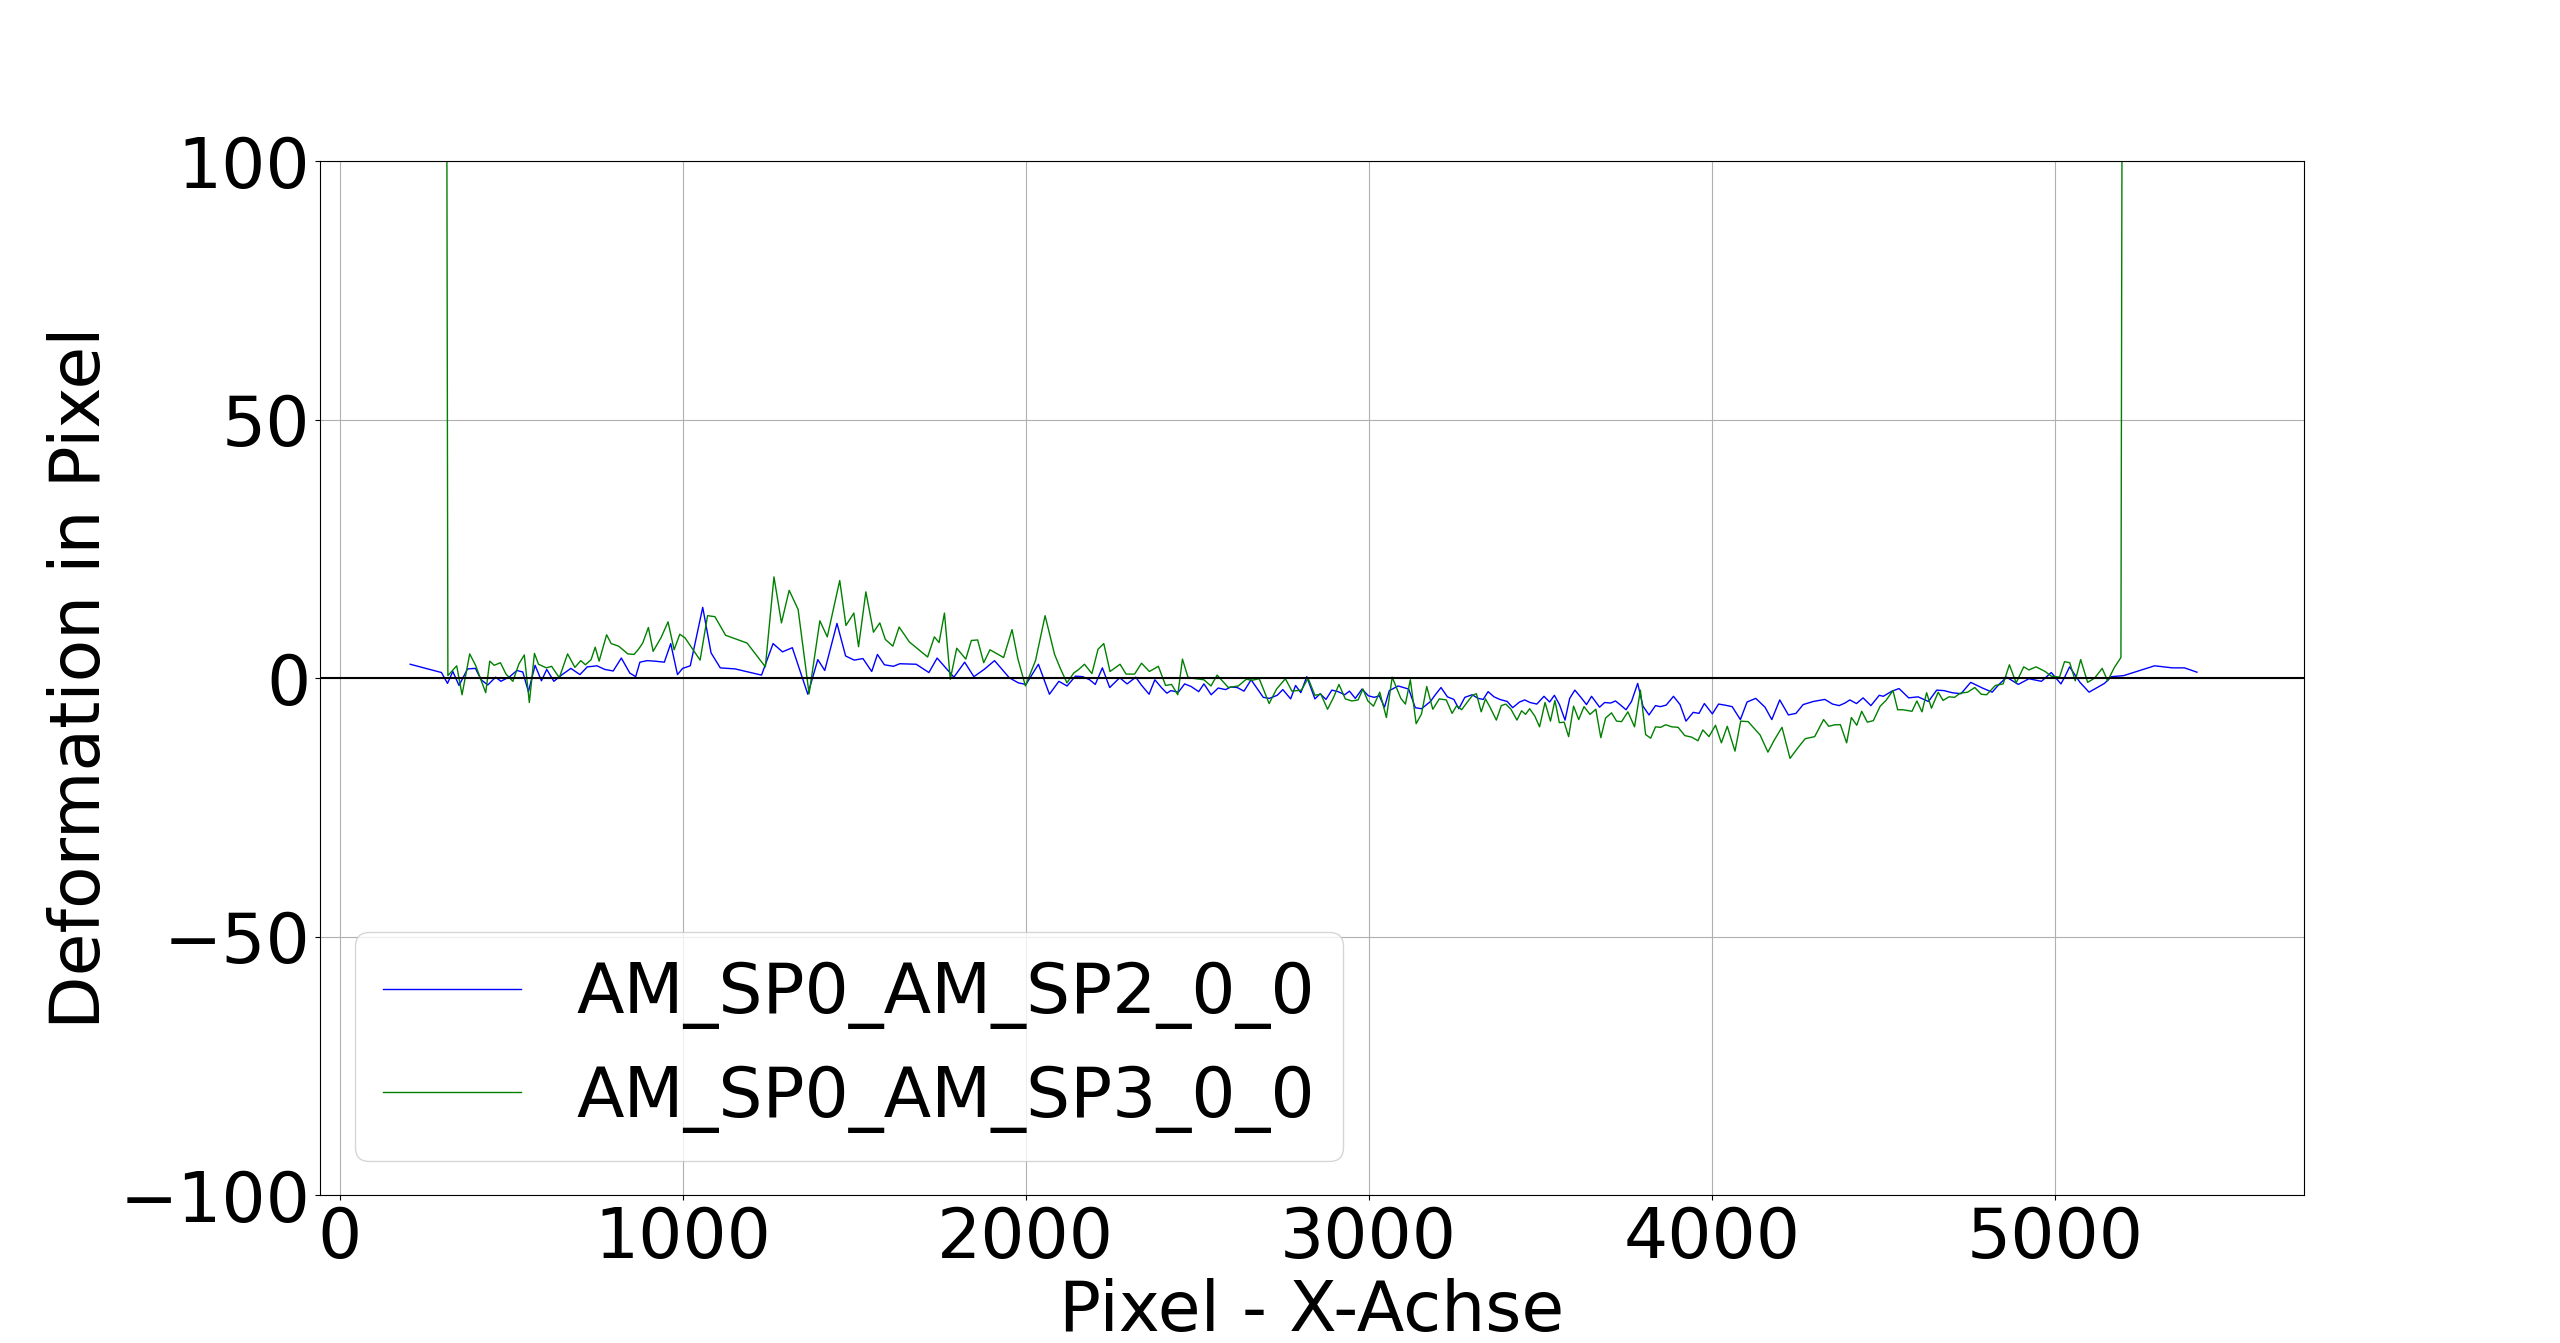
\includegraphics[width=0.9\textwidth]{images/AM_sp0_sp2_defo_plot.png}
    \caption{Differenz von mehreren Spannungsstufen bei einem AM Metall Bauteil}
    \label{fig:deformation_data_am}
\end{figure}

\subsection{Versuchsaufbau}

In Abbildung \ref{fig:versuchsaufbau} ist der Versuchsaufbau zur Datenerfassung 
zu sehen. Alle wichtigen Bestandteile sind nummeriert. Es folgt eine kurze Benennung
aller vorhandenen und notwendigen Teile:\\
1: Schraubstock Backen\\
2: Demonstratorbauteil\\
3: Scannerhalterung\\
4: Scanner LLT 30x0-25\\
5: Verschiebungsmesser\\
6: Laserlinie (Lila)\\
7: Schraubstock mit Kraftmesser\\
X: x-Achse\\
Y: y-Achse\\
Z: z-Achse\\

Der Scanner ist an dem Werkzeugkopf einer CNC-Fräse befestigt und wird 
in Richtung der X und Y Achse verschoben. So kann von dem kompletten Bauteil eine 
Pointcloud aufgenommen werden.

\begin{figure}[H]
    \centering
    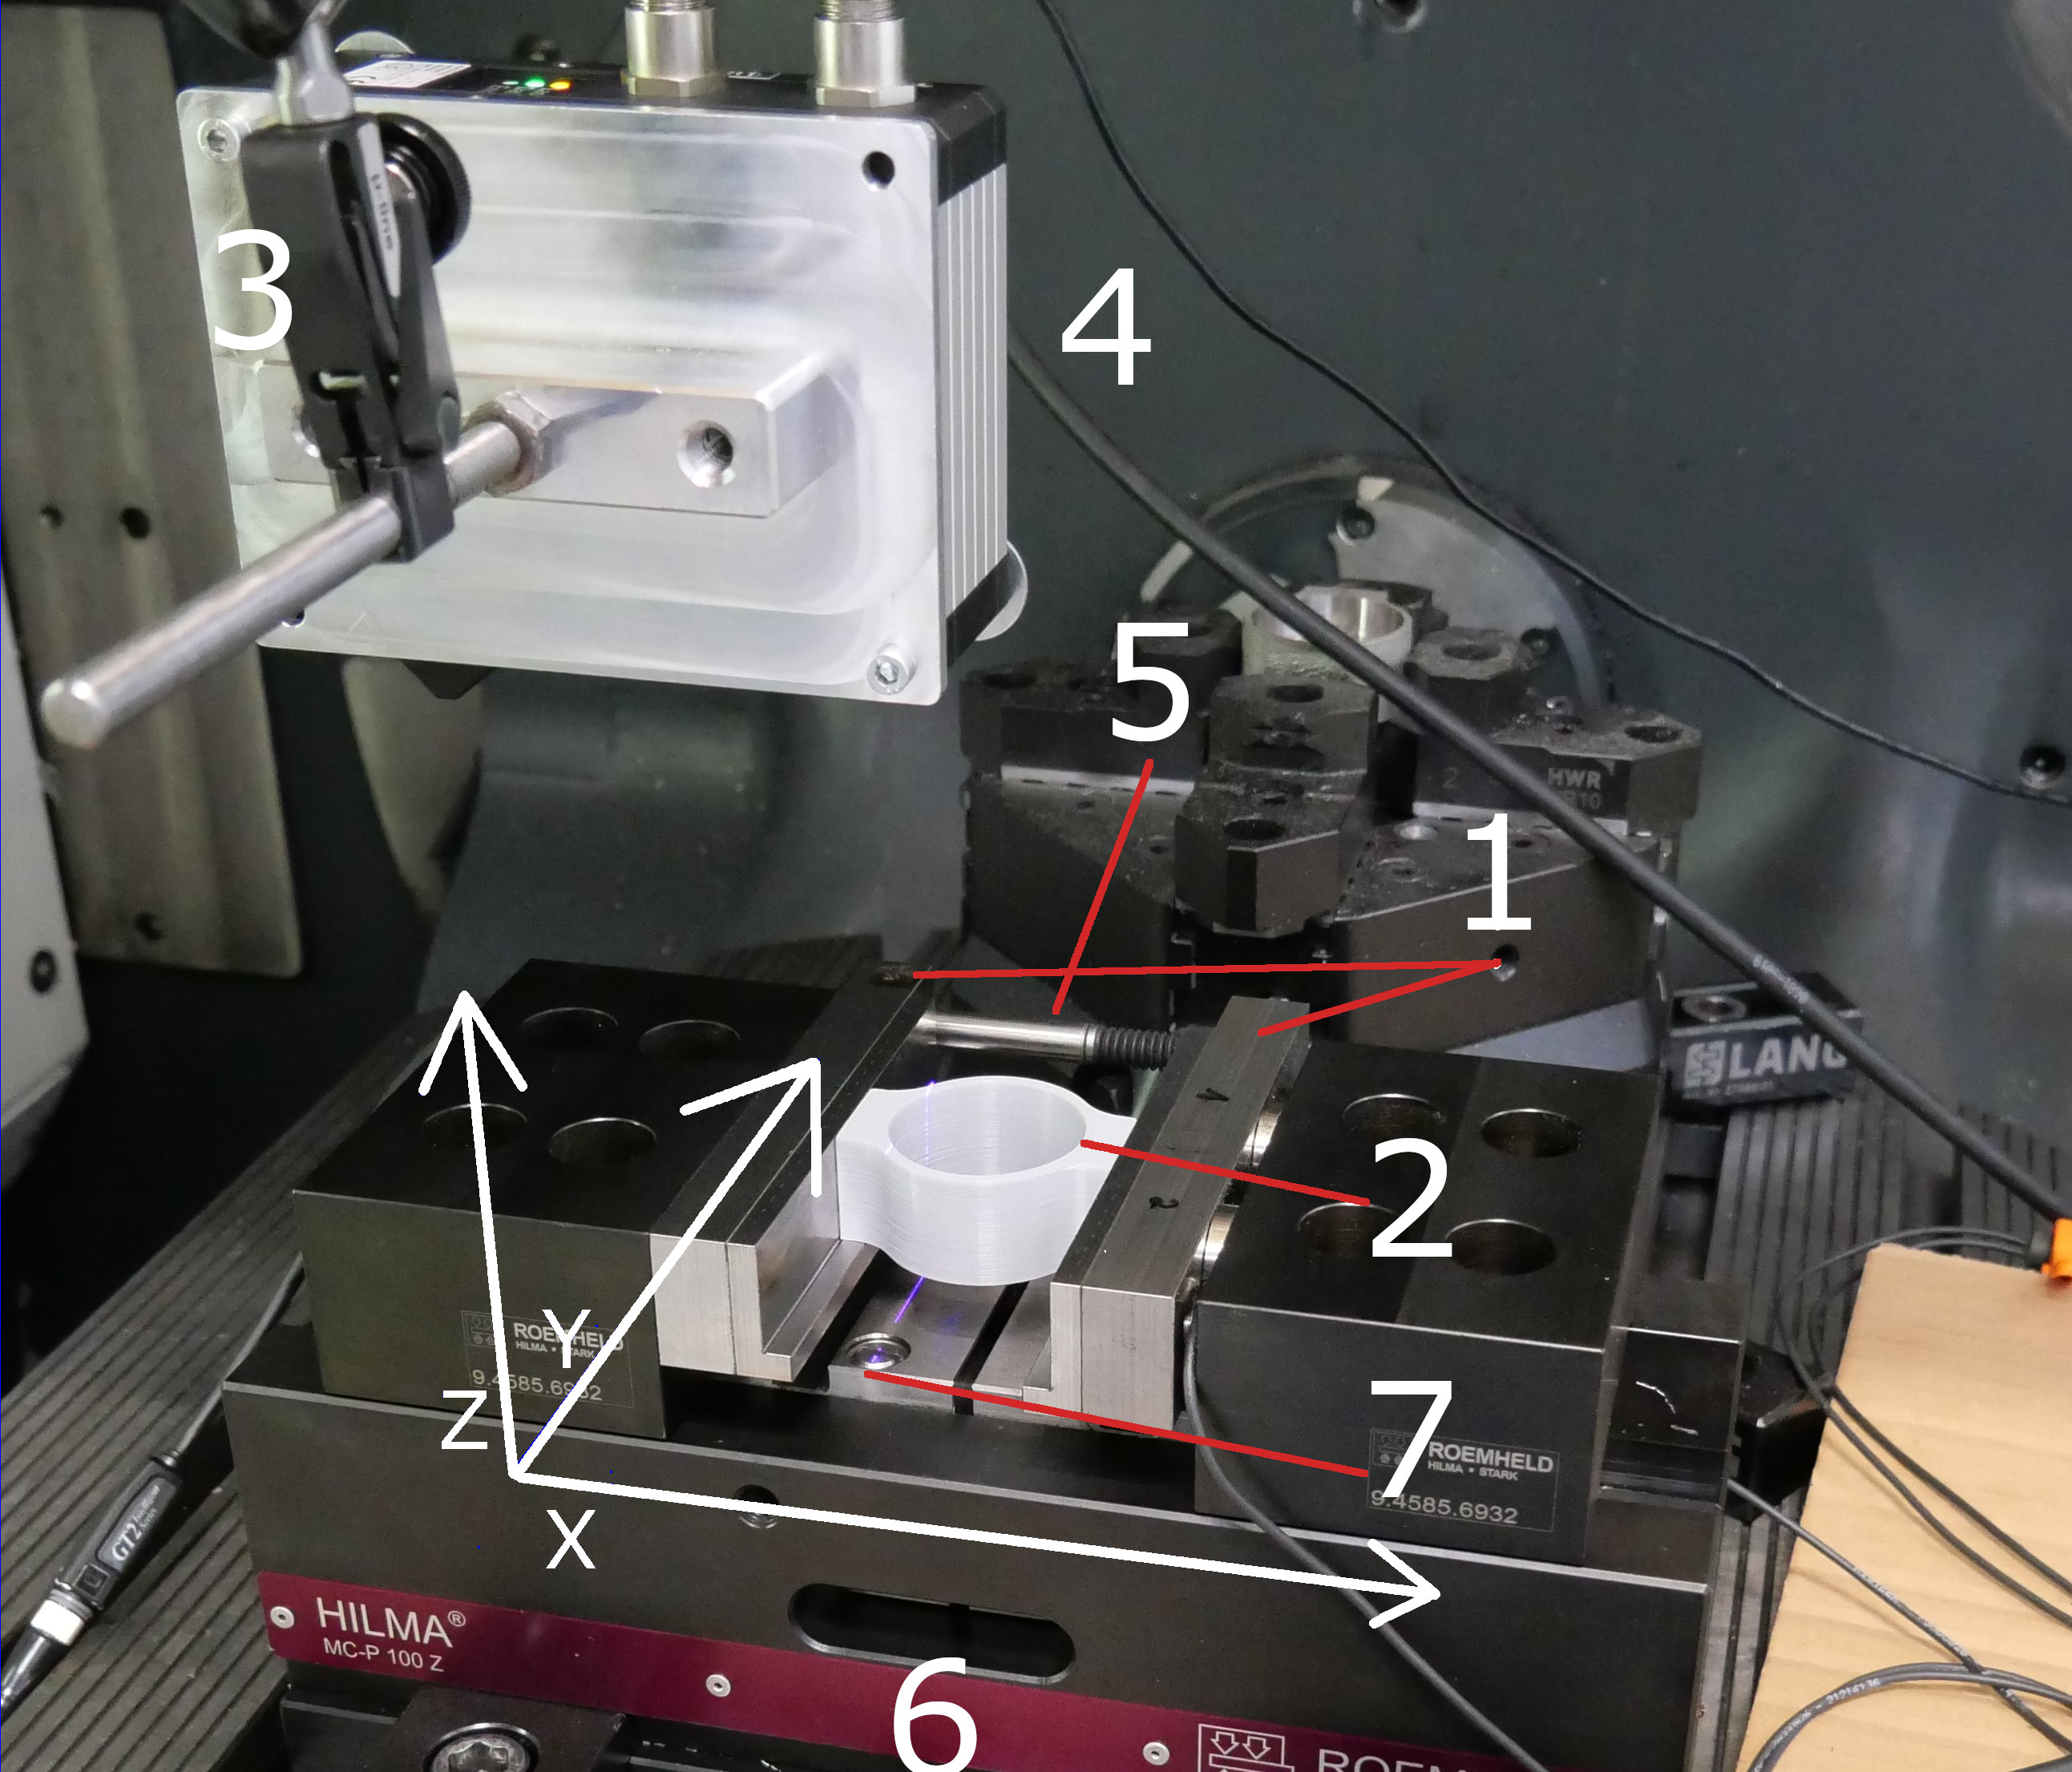
\includegraphics[width=0.6\textwidth]{images/versuchsaufbau_foto.png.JPG}
    \caption{Versuchsaufbau}
    \label{fig:versuchsaufbau}
\end{figure}

\section{Zusätzliche Messinstrumente}

Zusätzlich zu dem Scanner werden noch mit weiteren Messinstrumente Daten erfasst.
In Abbildung \ref{fig:versuchsaufbau} unter der Nummer 5 ist ein mechanischer 
Verschiebungsmesser zu sehen. Dieser misst die Verschiebung der Backen des 
Schraubstocks. Der Schraubstock misst zusätzlich mit viel Kraft die Backen 
aufeinander pressen.

Hierzu wird die piezoelektrische Kraftmesstechnik verwendet.
Bei Krafteinwirkung auf Piezokristalle (z. B. Quarz, Bariumtitanat, BaTiO3) 
werden im Kristallgitter negative gegen positive Gitterpunkte
verschoben, sodass an den Kristalloberflächen
Ladungsunterschiede Q als Funktion der Kraft F
gemessen werden.
Piezoelektrische Kraftaufnehmer sind mechanisch sehr steif, 
sie erfordern Ladungsverstärker
zur Messsignalverarbeitung und sind hauptsächlich zur Messung dynamischer Vorgänge
mit einer kleineren Frequenz als 1 Hz geeignet. \cite{Czichos.2020}. 
Diese Kraftmesstechnik ist 
für unseren Einsatzzweck gut geeignet da sie eine hohe Empfindlichkeit bietet 
und in vielfältigen Formen und Größen hergestellt werden kann. Zur Aufbereitung 
der Ladung, die der piezoelektrische Sensor, liefert wurde ein Ladungsverstärker 
eingesetzt.\cite{Schwartz.2006}
Dieser ist in Spannungsverstärker ist in Abbildung \ref{fig:taster} unten zu sehen.

\subsection{Messergebnisse}

Es wurden fünf Bauteile mit verschiedenen Spannungsstufen gemessen. Für jede 
Spannungsstufe wurde die Kraft, die auf das Bauteil wirkte sowie die Verschiebung 
des Schraubstocks gemessen.
Jede Spannungsstufe wurde durch Stufenweises anziehen des Schraubstocks erreicht.
Die Spannkraftkurve eines einzelnen Einspannvorgangs ist in 
Abbildung \ref{fig:single} zu sehen. 
In der Spannungskurve ist ein elastischer Bereich für das 
Bauteil zu sehen, in dem sich die Spannkraft zurückbewegt, nachdem kein 
Anzugdrehmoment mehr anliegt. Aus diesem Grund kann nicht der maximale Wert der Spannkraft angenommen werden, 
sondern es muss ein Wert gewählt werden der nach dem maximalen Ausschlag liegt.
Dieser wurde über die erste Ableitung der Spannkraftkurve gefunden. Sobald der 
Absolutwert der Steigung unter 0.0009 N fällt, wir die Spannkraft und Auslenkung an 
diesem Punkt gewählt. 0.0009 N wurde empirisch ermittelt um bei allen Bauteilen einen 
angemessenen Wert zu liefern.
Die Spannkraft wurde an zwei Achsen aufgenommen und zu der Gesamtkraft aufsummiert.

\begin{figure}[H]
    \centering
    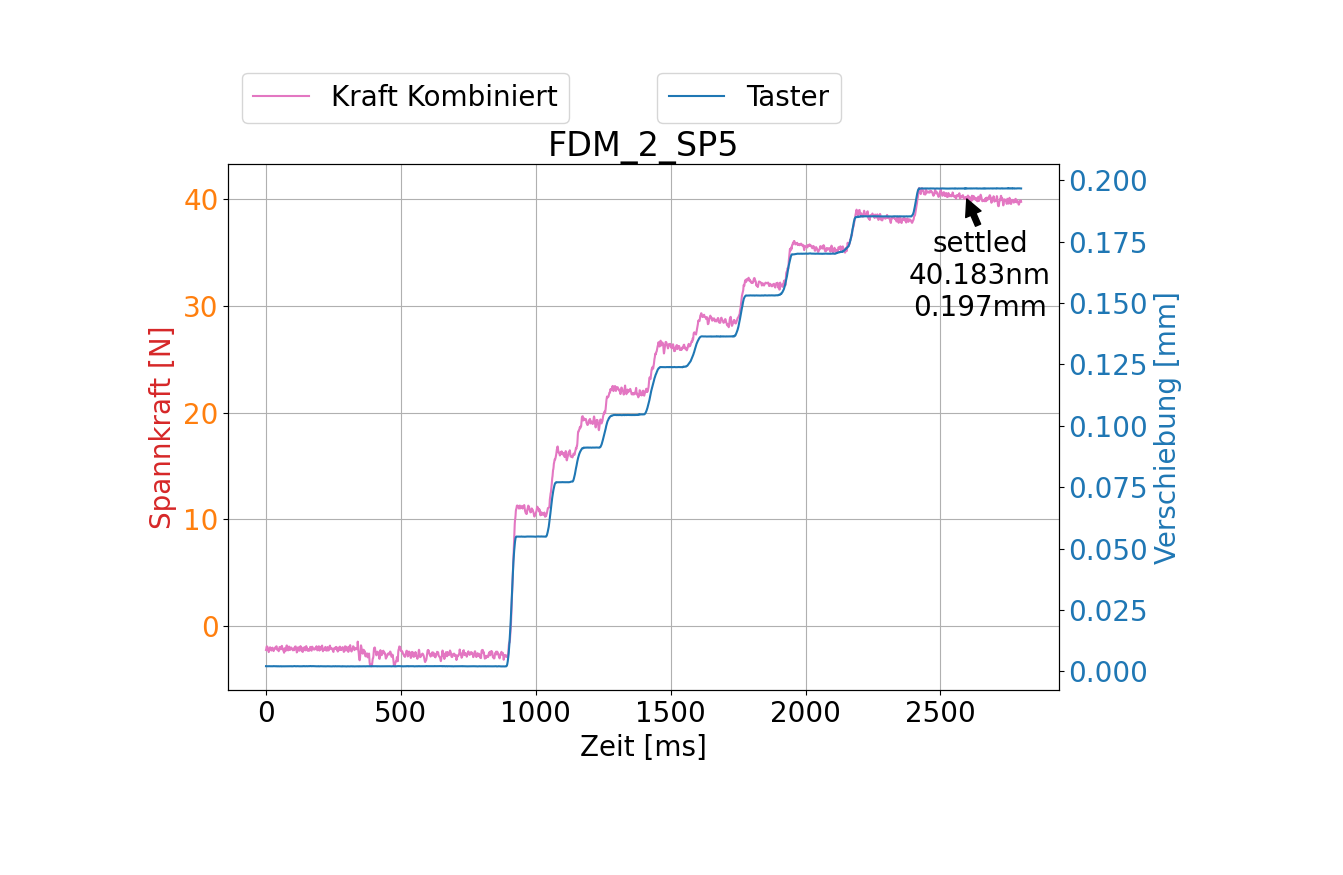
\includegraphics[width=0.99\textwidth]{images/spannkraftstufen_single.png}
    \caption{Kraft- und Verschiebung der Spannungsstufe fünf bei einem FDM Bauteil}
    \label{fig:single}
\end{figure}

Diese maximalen Werte für die Spannkraft und Auslenkung wurden für jedes Bauteil 
akkumuliert und sind in Abbildung \ref{fig:akkumulated} dargestellt.
Die mit dem FDM Prozess hergestellten Bauteile wurden mit jeweils sechs Spannungsstufen 
gemessen. Zwischen jeder Stufe wurde versucht eine konstante Kraft auf das Bauteil 
auszuüben. Durch den händischen Prozess des anziehen des Schraubstocks war die jedoch 
nicht immer möglich. 
Die Metallbauteile unterscheiden sich durch ihren Aufbau. Alle basieren auf dem gleichen
3D-Modell, besitzen jedoch Änderungen in der Stützstruktur.
In dem Bauteil AM0 ist die volle Stützstruktur vorhanden, in den Bauteilen 
AM1 und AM2 wurde die Stützstruktur mit einem Bohrer in verschiedener Tiefe
ausgebohrt. Die Bauteile sind in Abbildung \ref{fig:am_parts} dargestellt.

Das Bauteil AM0 wurde nur mit zwei Spannungsstufen gemessen, da schon bei der zweiten 
Stufe über 2500 nm Kraft erforderlich war, um das Bauteil nur minimal in x-Richtung 
zu deformieren. Das ist zeigt, dass die Stützstruktur sich stark auf die Verformbarkeit
eines Bauteils auswirkt. Bei dem Bauteil AM1 wurden 2500 nm nach vier Spannungsstufen 
erreicht. Wenn man die Verformung in x-Richtung mit der Verformung von AM2 vergleicht, 
ist zu sehen, dass das Bauteil ohne Stützstruktur etwa doppelt so weit, bei einer 
ähnlichen Kraft, in x-Richtung deformiert wurde.

Die FDM Bauteile wurden mit deutlich weniger Kraft eingespannt. Hier wurde bei ca. 
250 nm gestoppt, dennoch ist die Verschiebung der Teile deutlich höher als bei den 
AM Teilen. Diese Werte wurden aufgenommen um die Visuelle Deformationserkennung zu 
validieren.

\begin{figure}[H]
    \centering
    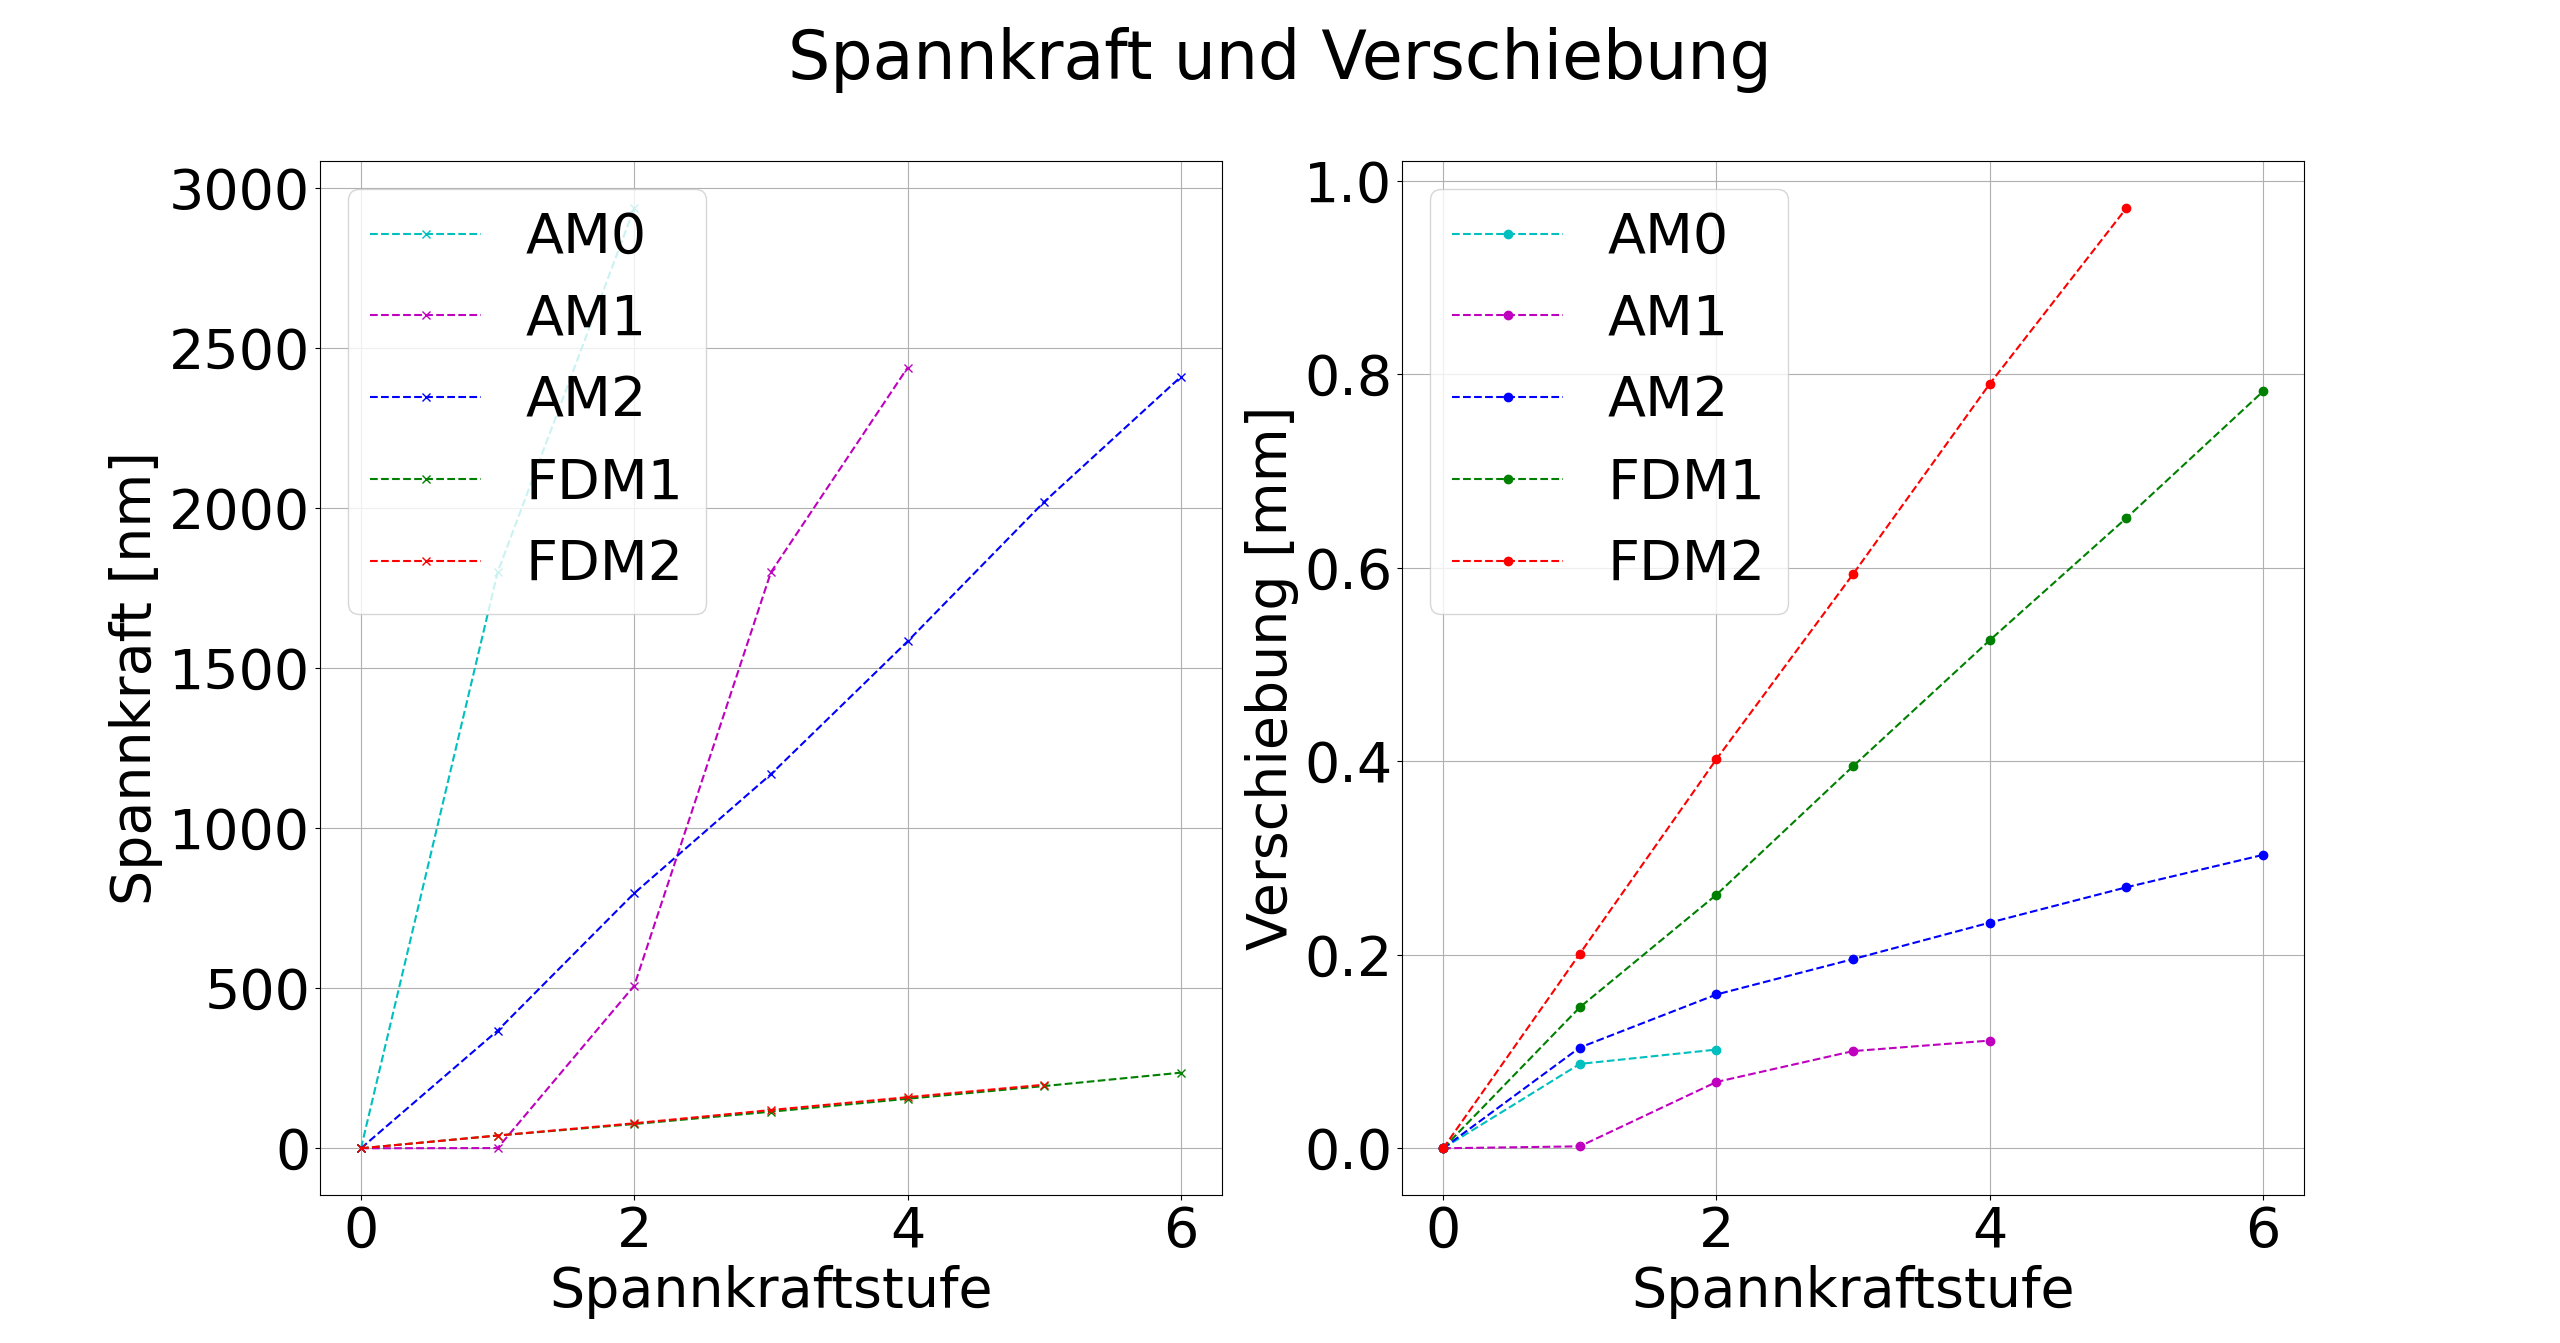
\includegraphics[width=0.99\textwidth]{images/spannkraftstufen_akkumuliert.png}
    \caption{Akkumulierte Kraft- und Verschiebung jedes Bauteils}
    \label{fig:akkumulated}
\end{figure}

\begin{figure}[H]
    \centering
    \begin{minipage}{.33\textwidth}
      \centering
      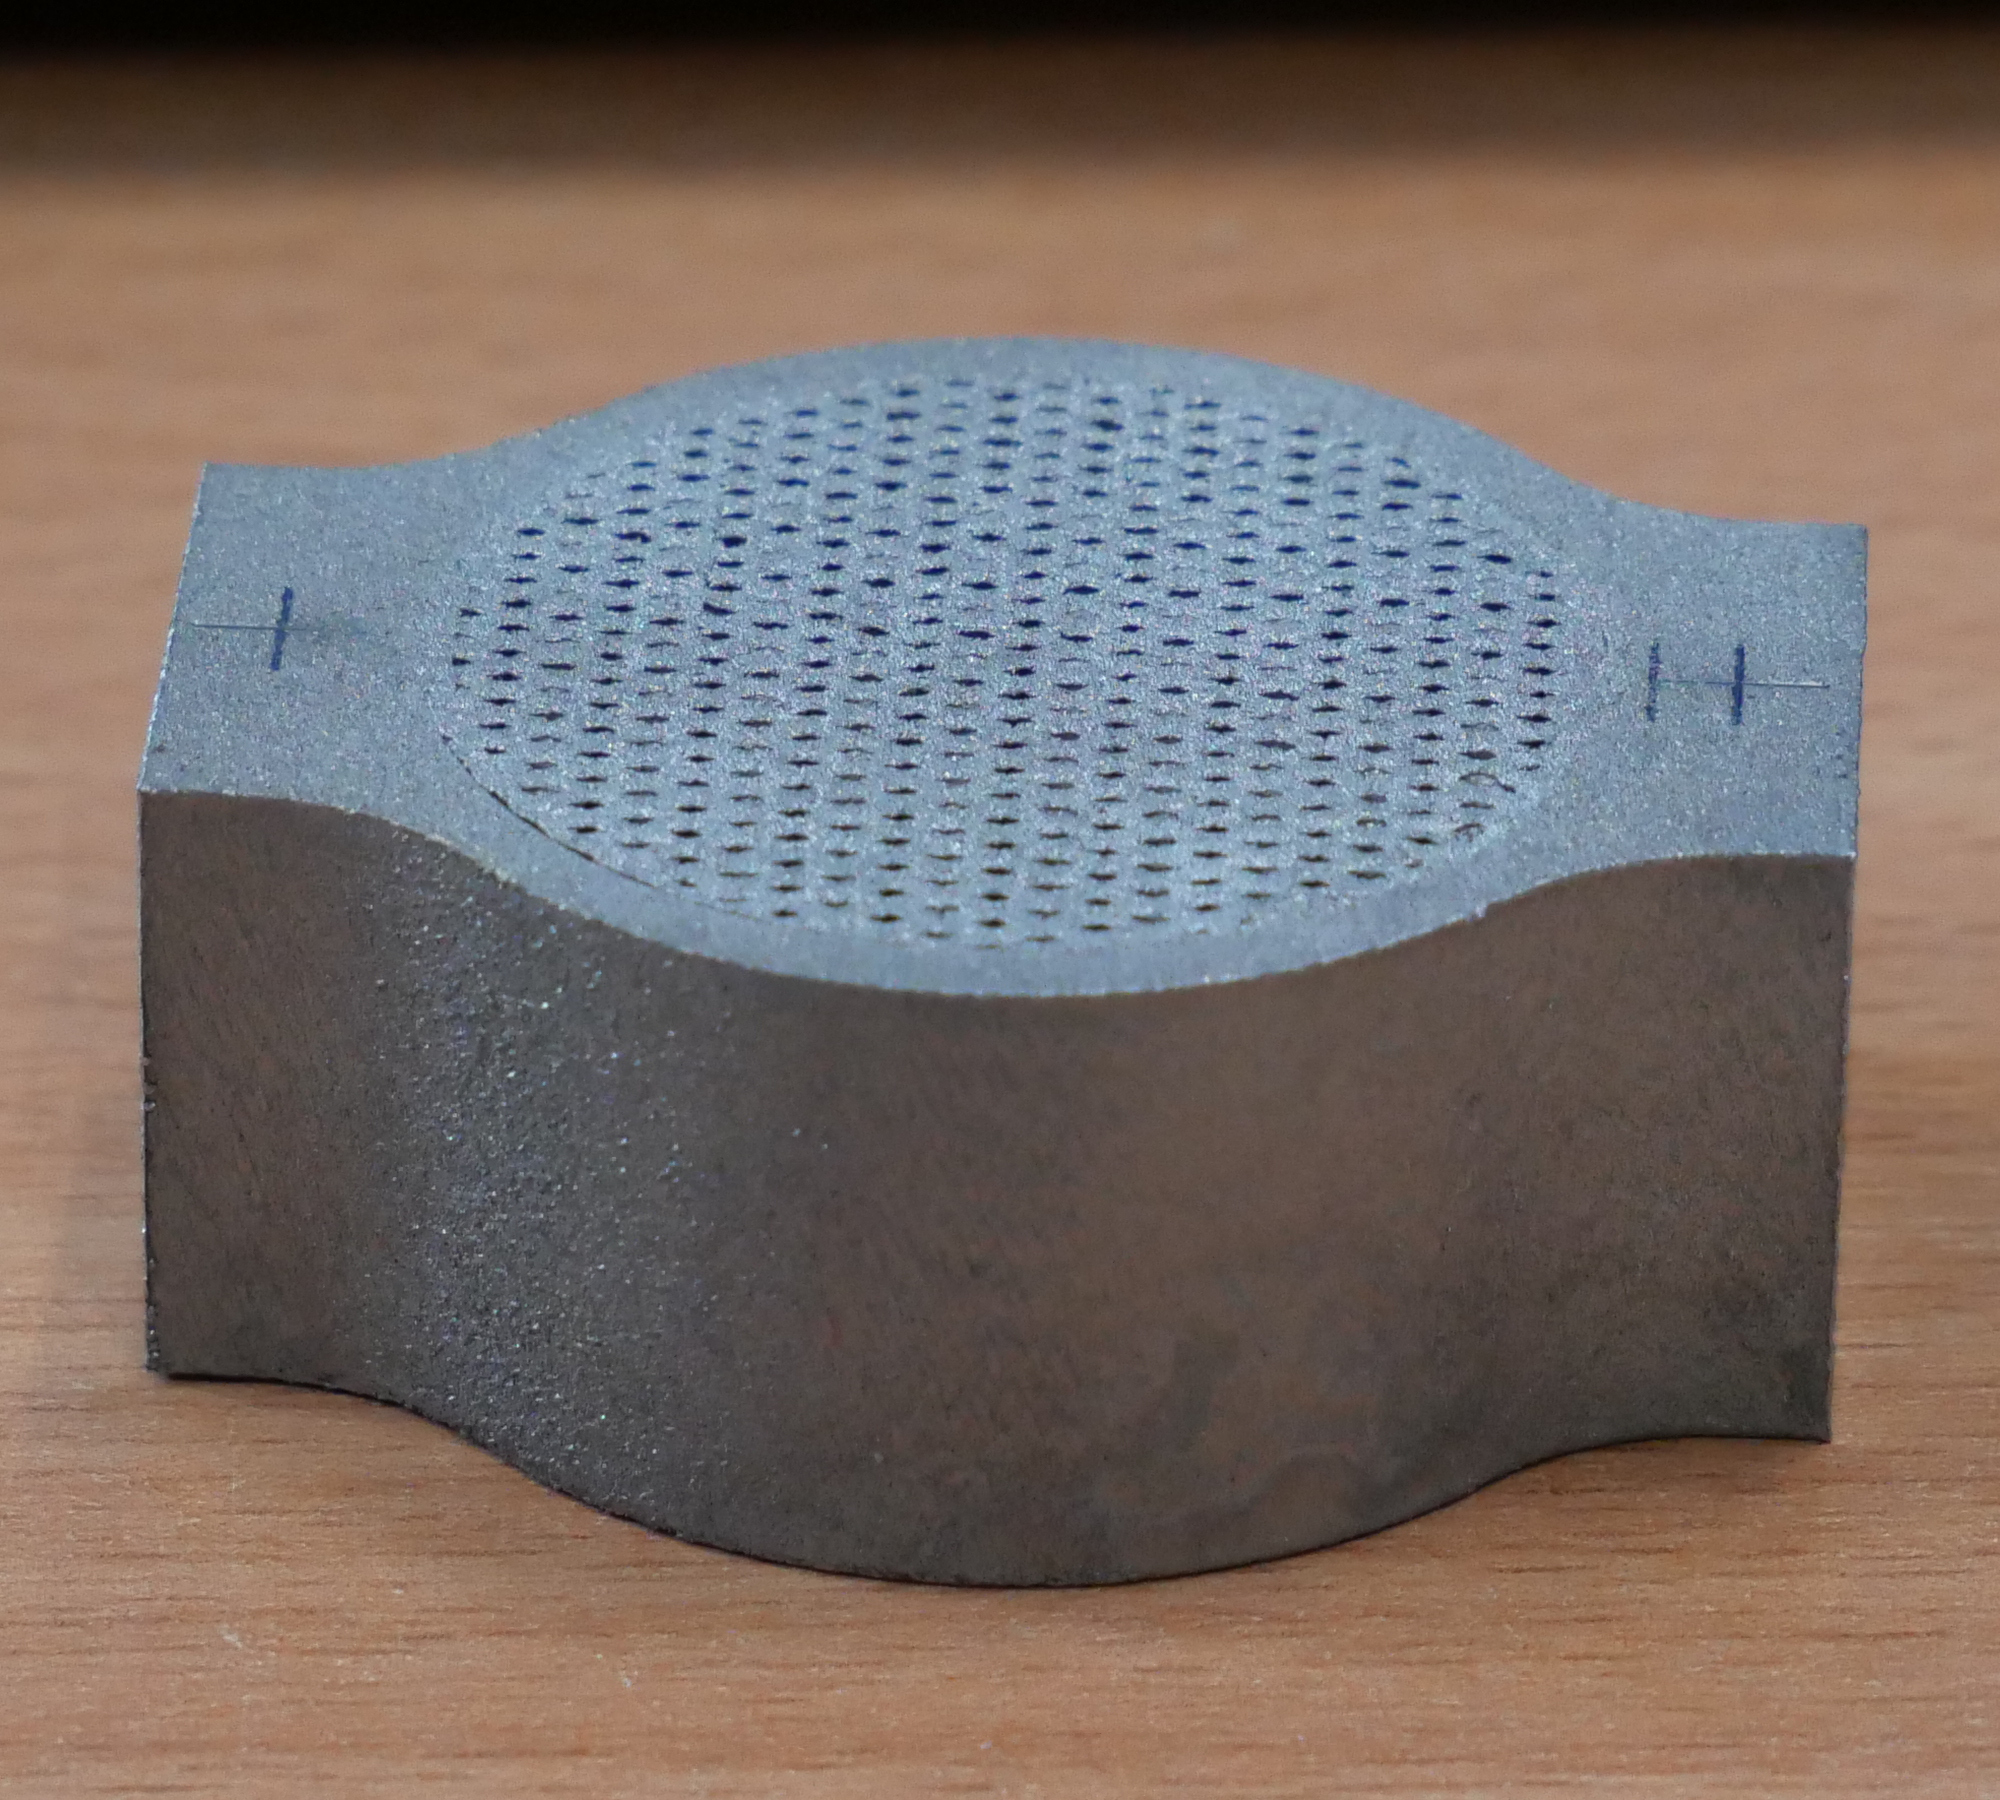
\includegraphics[width=0.9\linewidth]{images/AM0_crop.JPG}
      \caption*{(a)}
    \end{minipage}%
    \begin{minipage}{.33\textwidth}
      \centering
      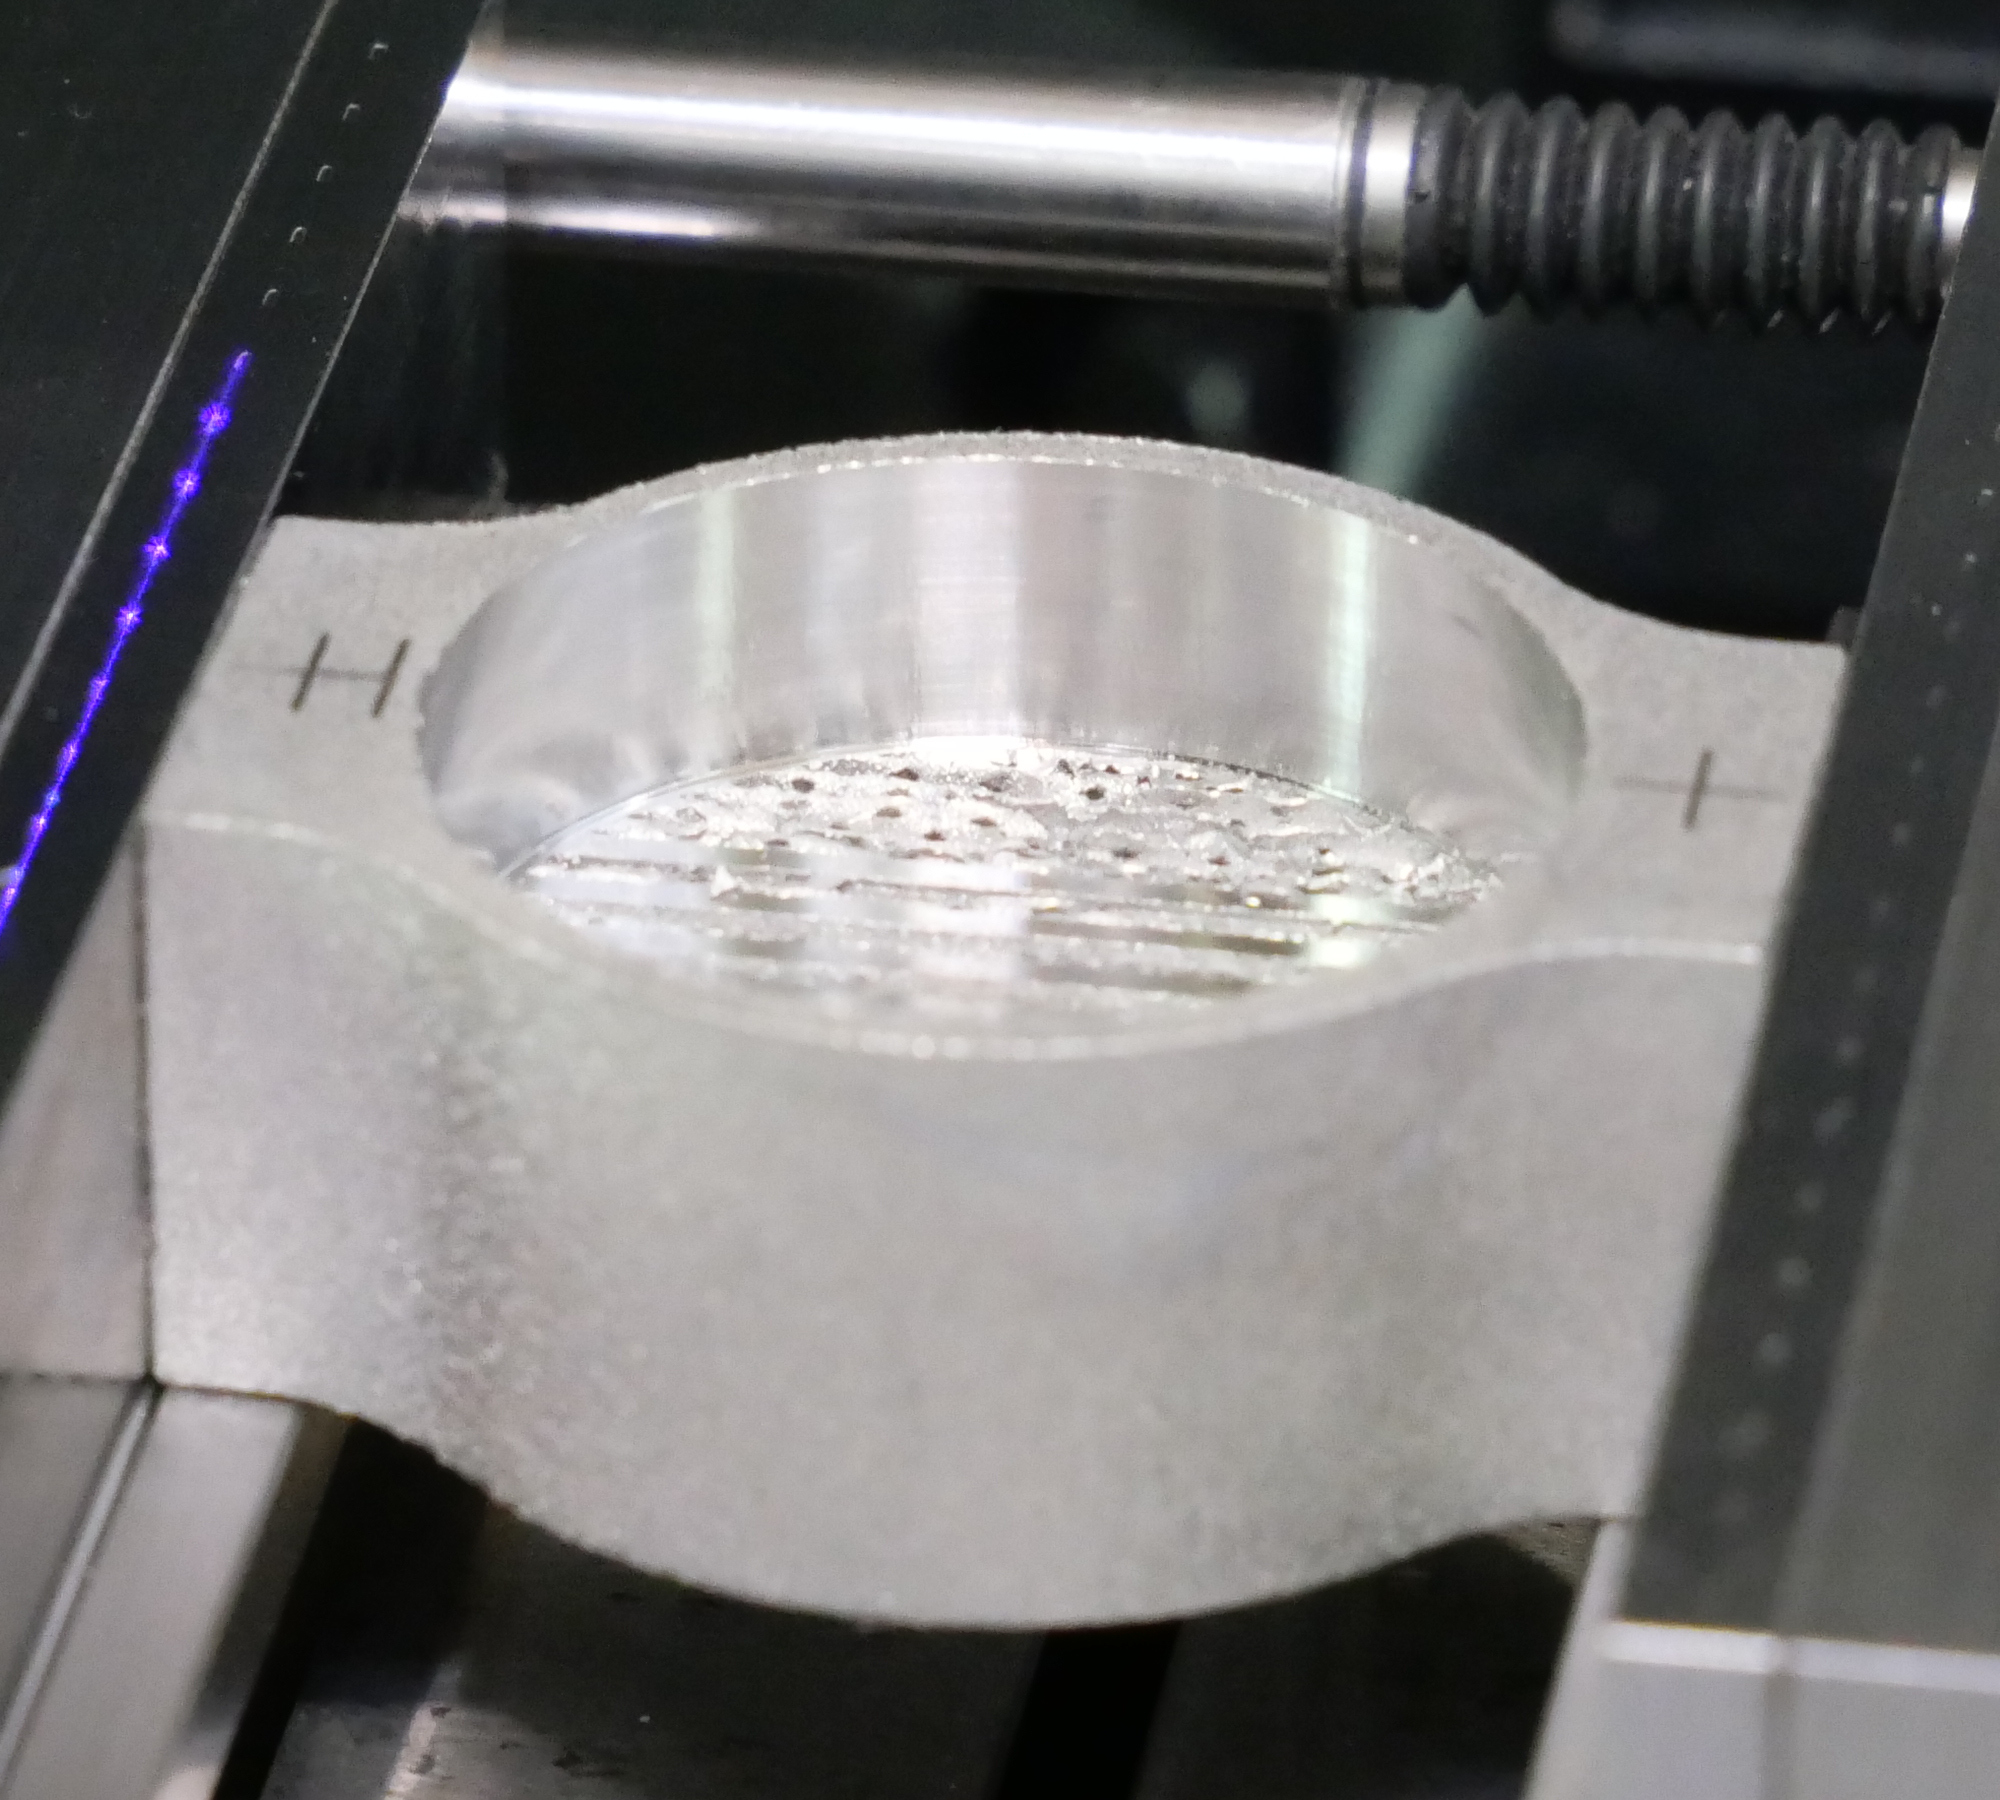
\includegraphics[width=0.9\linewidth]{images/AM1_crop.JPG}
      \caption*{(b)}
    \end{minipage}
    \begin{minipage}{.33\textwidth}
        \centering
        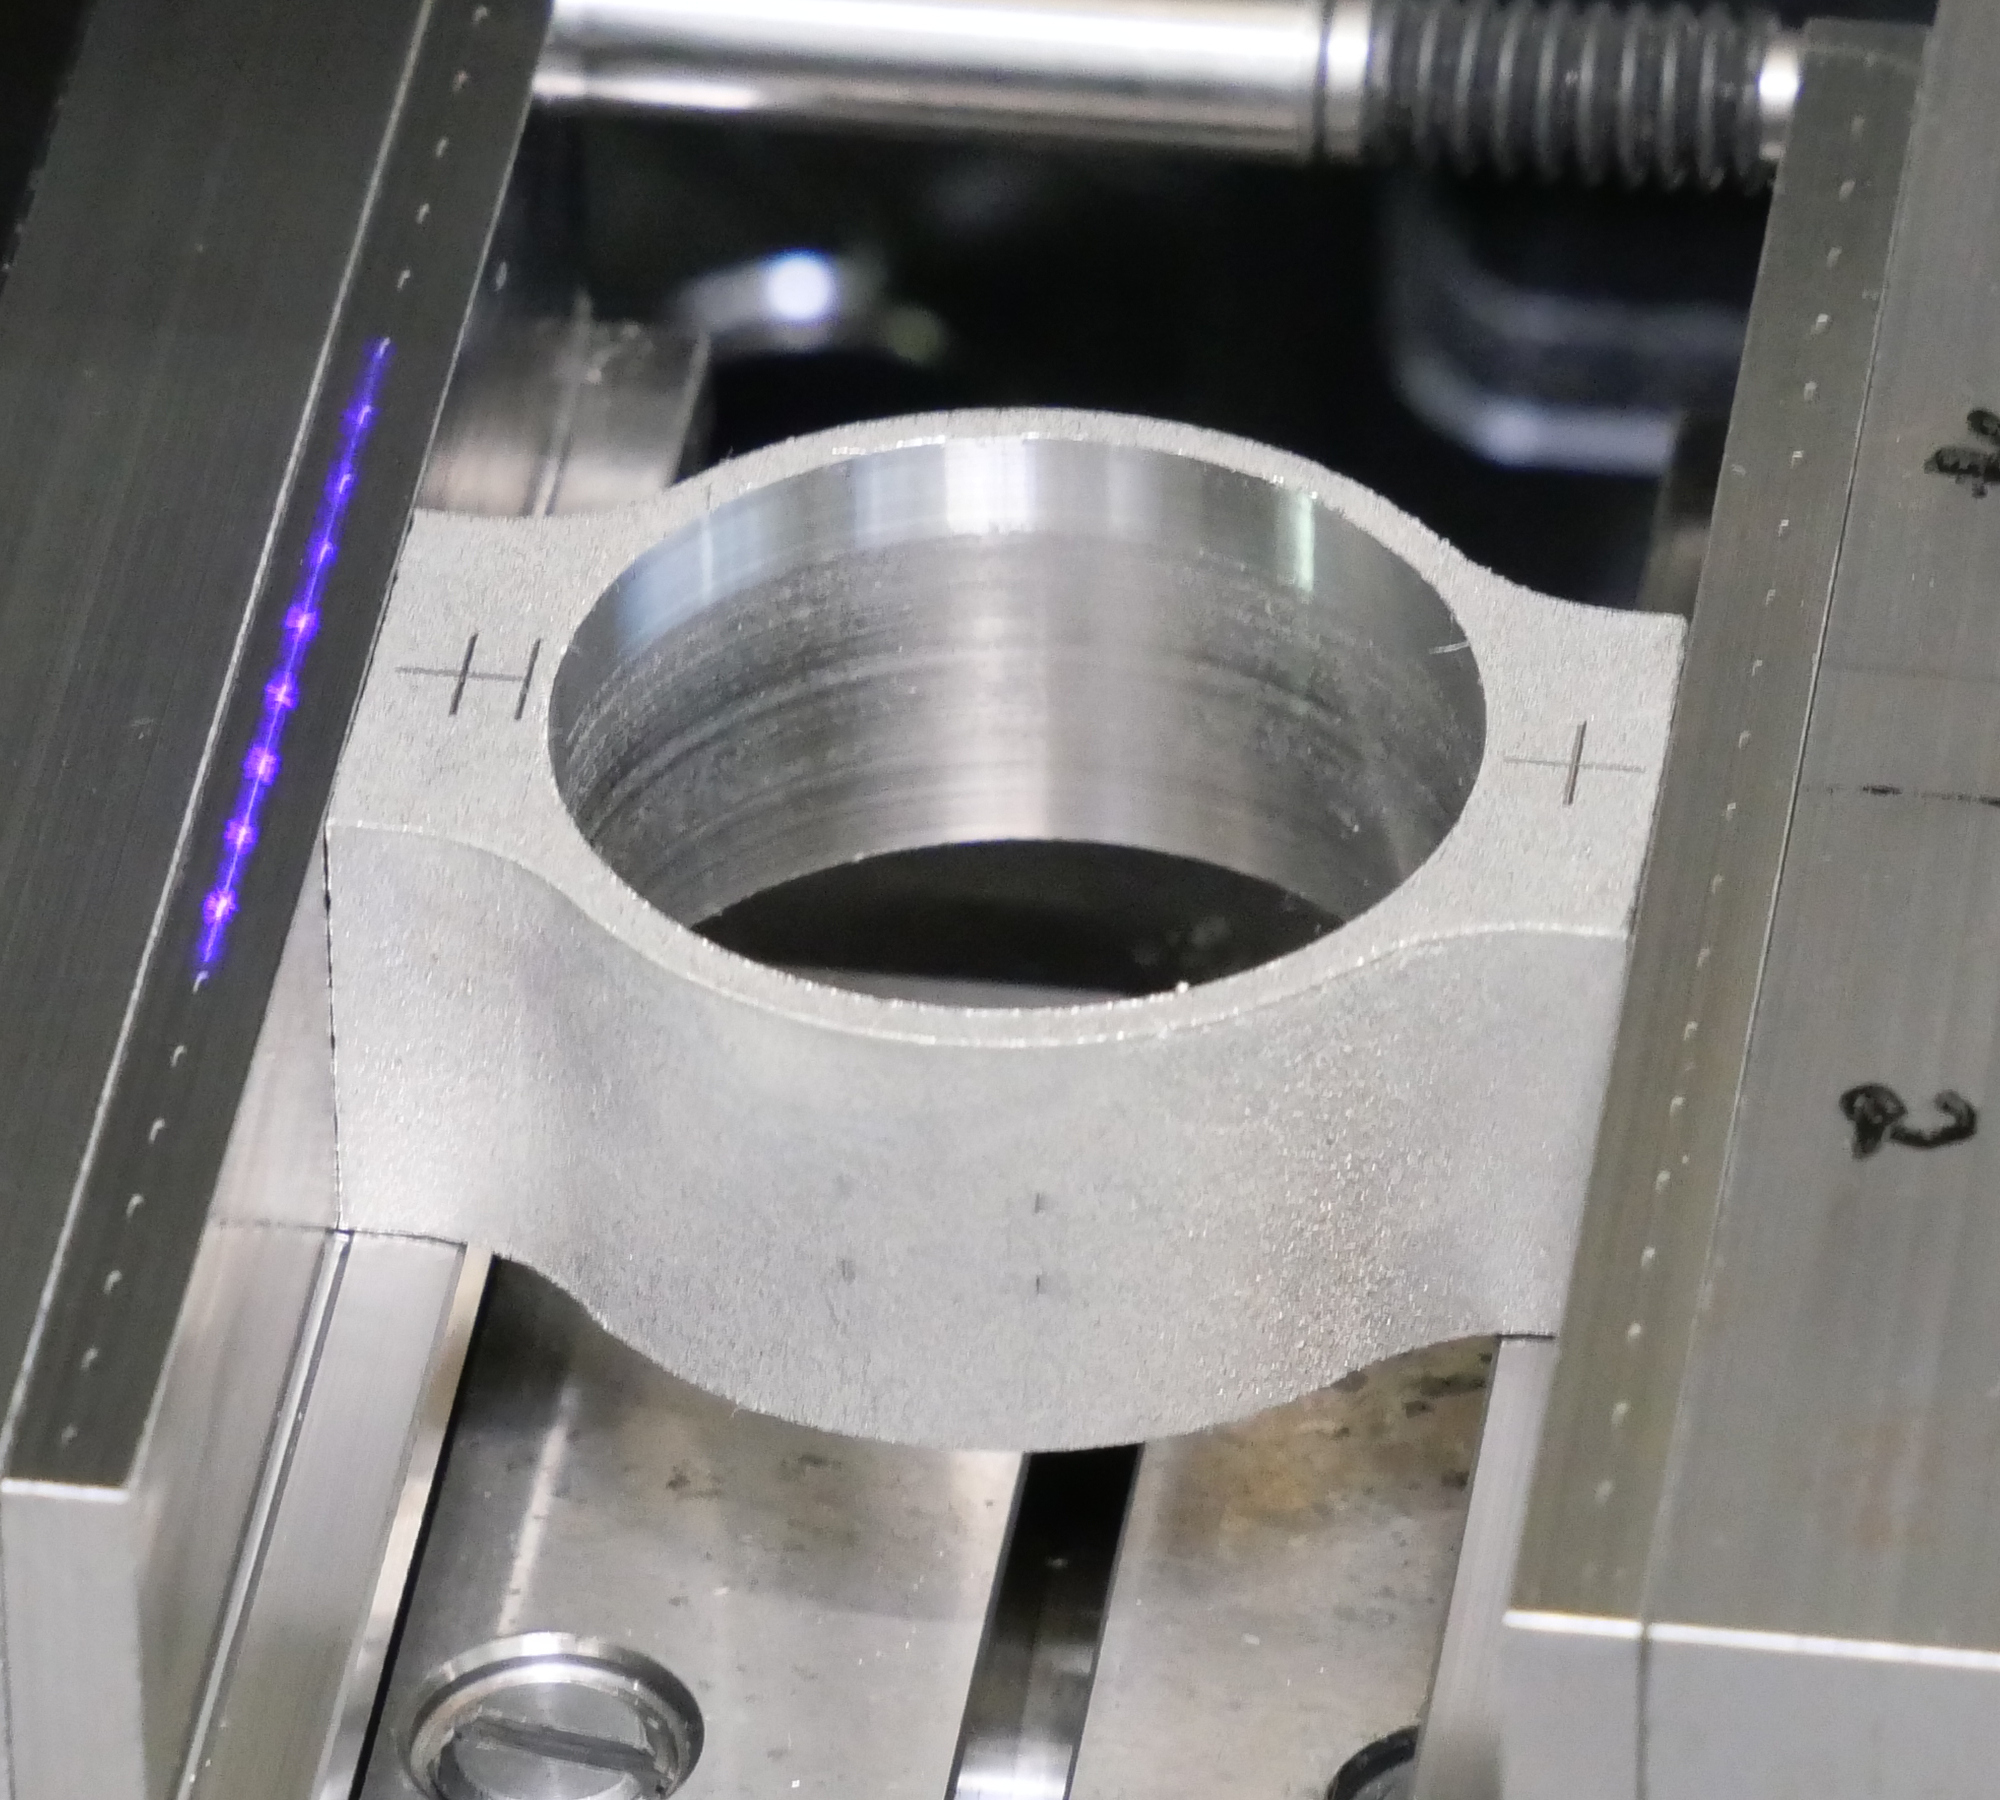
\includegraphics[width=0.9\linewidth]{images/AM2_crop.JPG}
        \caption*{(c)}
      \end{minipage}
      \caption{(a): AF Metallbauteil mit voller Stützstruktur, Bezeichnung: AM0.
      (b): AF Bauteil mit der halben Stützstruktur ausgebohrt, Bezeichnung: AM1.
      (c): AF Bauteil ohne Stützstruktur, Bezeichnung: AM2}
      \label{fig:am_parts}
\end{figure}
    
Zusätzlich werden die Bauteile nach einem Scanvorgang mit einem Taster 
abgetastet. Hierfür wird der Werkzeugkopf gewechselt und der Scanner entfernt.
Dann wird der Taster in die CNC-Maschine eingesetzt und das Bauteil abgetastet.
In Abbildung \ref{fig:taster} ist das Tasterwerkzeug zu sehen. Die rote Kugel 
am Ende des Tasters erkennt, sobald eine Berührung zu dem Bauteil erfolgt ist 
und benachrichtigt den Steuerungsrechner. Dieser speichert die aktuelle Position 
dann in einer Protokolldatei. Durch diese Daten kann die Deformation auch an 
den Randbereichen der Bauteile validiert werden.